\chapter{H\"older Conjecture} 
% 
% The complexity coefficients were designed, as their name implies, to capture the complexity of a times series. 

In this chapter, we explore how the complexity coefficients relate to other characteristics of time series. In particular, we use a number of simulations to examine the relationship between the complexity coefficients and both the H\"older class of a function and the fractal dimension of the function's graph. We begin by looking the behavior of
the complexity coefficients for a few simple functions with added noise. The complexity coefficients are given by parameters of $\log-\log$ linear fit to points whose original values is less than 1 and the interpretation of the parameters may not be intuitive. These simple examples are meant to orient the reader in interpreting some aspects of the complexity coefficients.  

% value of the complexity coefficients for a few 
% simple functions. 

\section{The Complexity Coefficients}
In the theoretical development of $\varepsilon-$complexity, 
the continuous function to be analyzed was assumed to on 
the interval $[0,1]$. Here we refer instead to the index
of the samples of the function which, like the time 
parameter of a time series, are in $\{ 1,2,3,.... \}$.
The complexity coefficients are computed by finding the best approximation to a function as that function is downsampled by integer amounts, that is, points indexed by $h\N$ are used in the reconstruction. In our implementation of the algorithm, a function is downsampled at $h \in \{ 2,3,4,5,6 \}$ giving us 
five downsampling levels. The minimal approximation error, $\varepsilon_h$ is computed for each level $h$. We denote the  proportion of the samples retained $\mathbb{S}_h = \frac{1}{h}$.
The $\varepsilon-$complexity coefficients $A, B$ are then result of an ordinary least squares fit: 
\[
     \log(\varepsilon_h) = A + B \mathbb{S_h}.
\]


\begin{figure}[h]
  \begin{subfigure}[b]{0.45\textwidth}
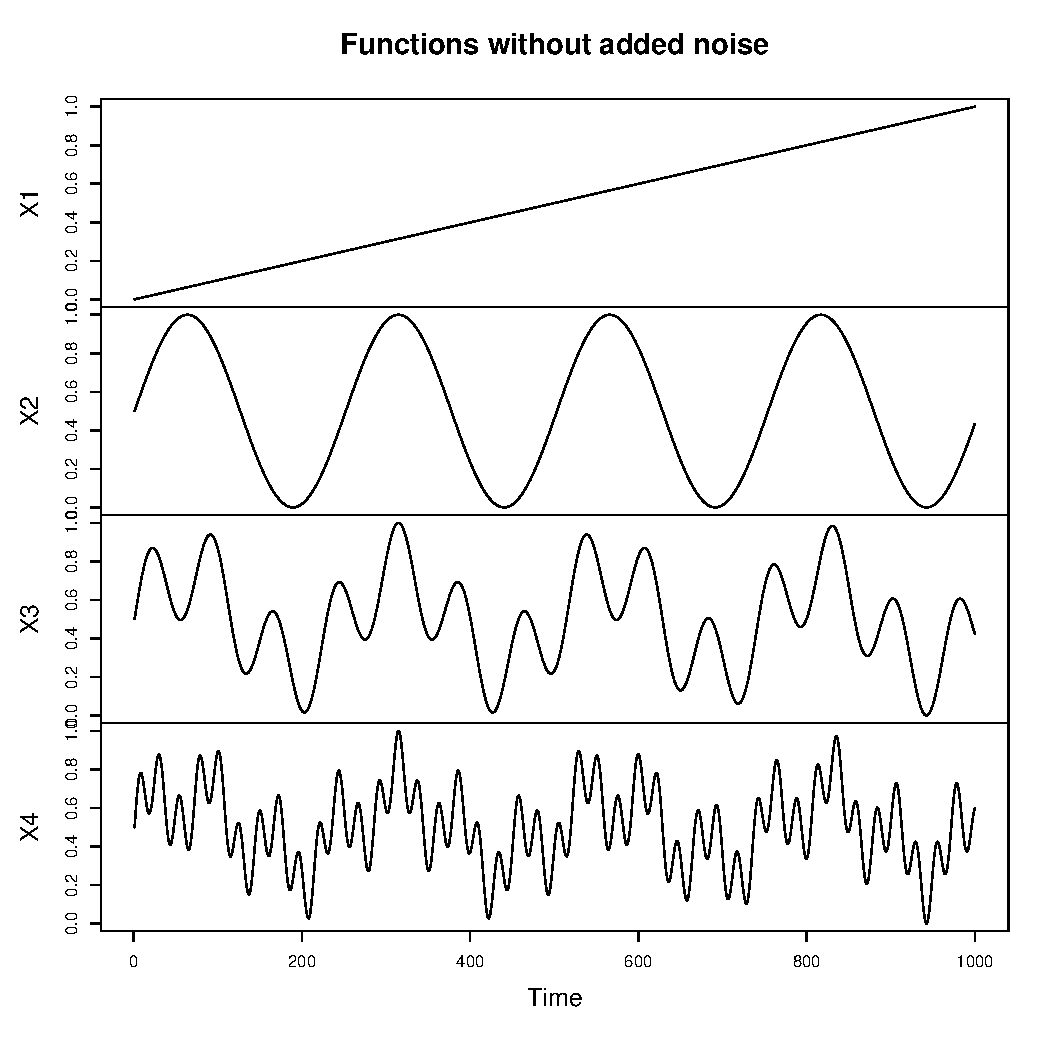
\includegraphics[width = 0.9\linewidth, height = 3in]{./figs/coeff-interp-simple-functions0.pdf}
    % \caption{Functions without added noise.}
    % \label{fig:simple-functions1}
  \end{subfigure}
  \hfill
  \begin{subfigure}[b]{0.45\textwidth}
  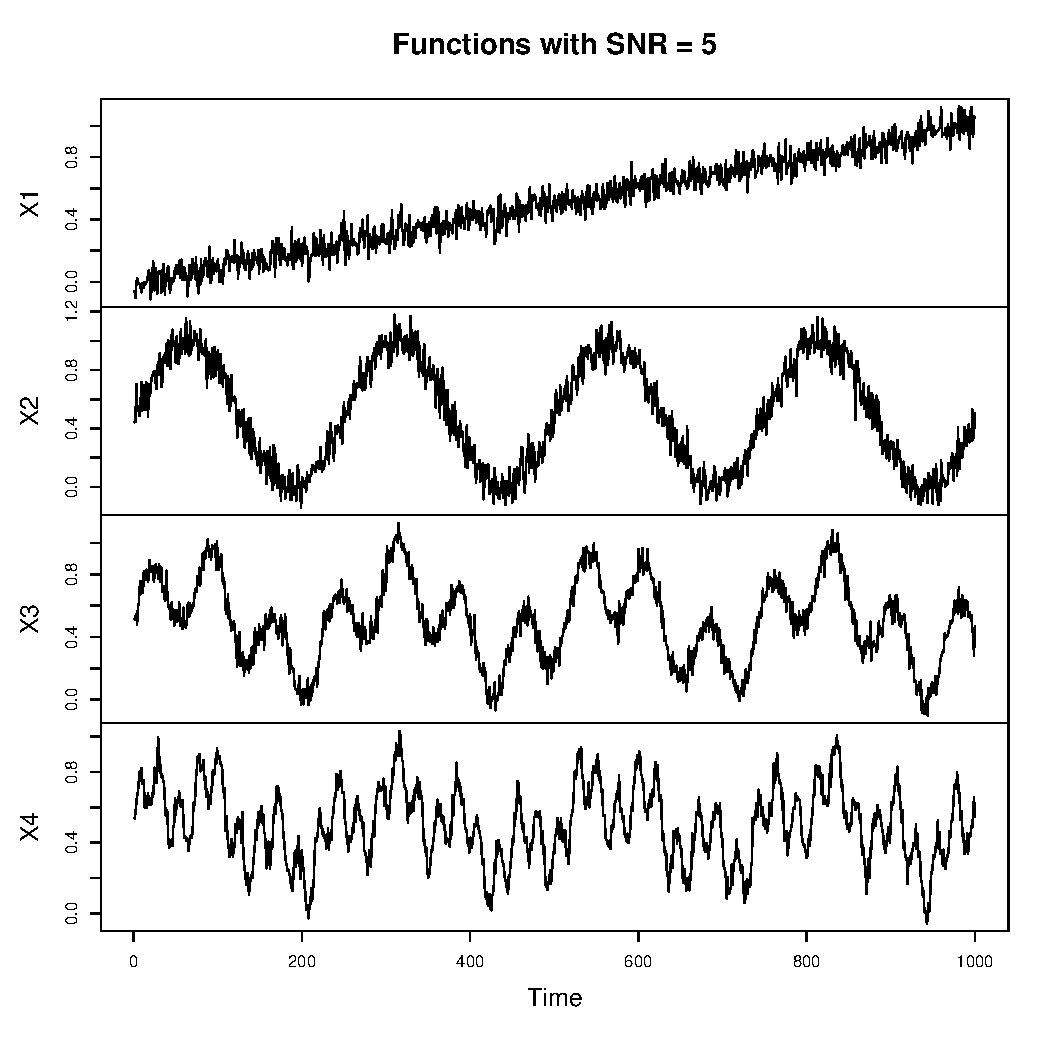
\includegraphics[width = 0.9\linewidth, height = 3in]{./figs/coeff-interp-simple-functions1.pdf}
  % 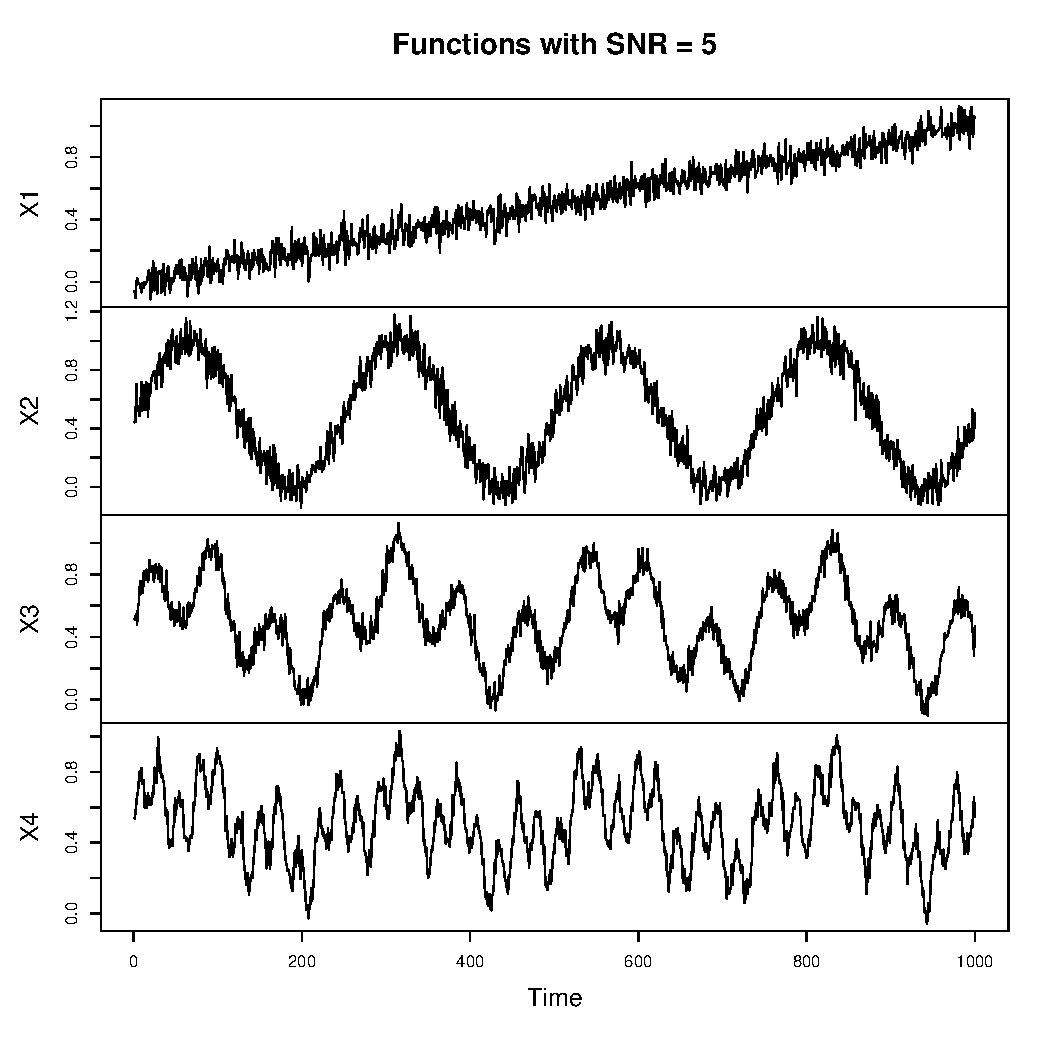
\includegraphics[width = 0.9\linewidth, height = 3in]{./figs/coeff-interp-simple-functions1.pdf}
    % \caption{Functions without added noise.}
  \end{subfigure}
  \caption{Simple linear and sinusoidal functions with and 
  without added noise.}
     \label{fig:simple-functions}
\end{figure}

  \begin{figure}[h]
    \begin{center}
    % \begin{picture}(60,60)
    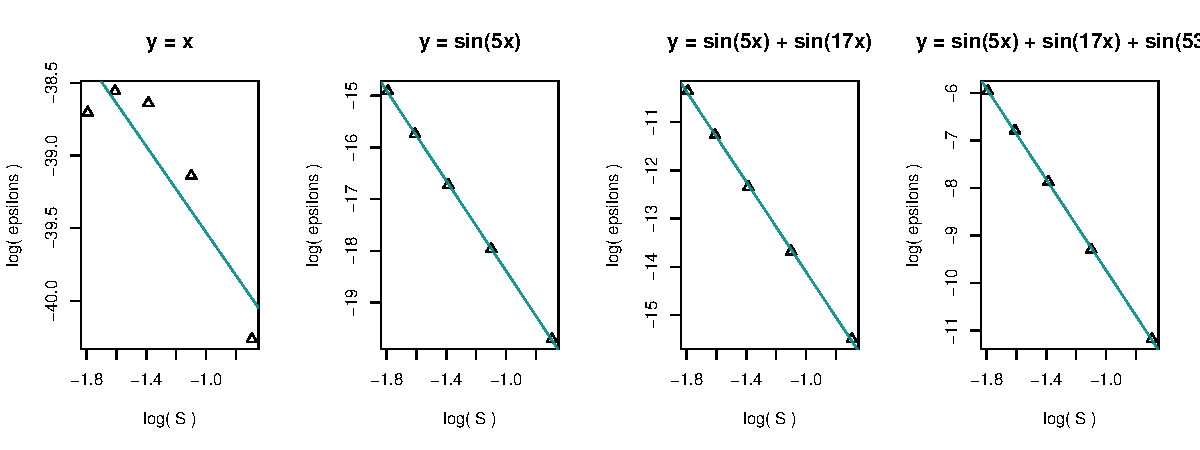
\includegraphics[width = \textwidth, keepaspectratio]
    {./figs/coeff-interp-simple-fits.pdf}
    % \end{picture}
    \end{center}
    \caption{The log-log linear fit of the approximation errors 
    against the proprotion of points $\mathbb{S}_h$ used to 
    approximate the functions \ref{fig:simple-functions}}.
    \label{fig:simple-fits}
  \end{figure}

% \begin{figure}[!htbp]
%   \begin{center}
%   % \begin{picture}(60,60)
%   \includegraphics[totalheight = 3.4in]
%   {./figs/coeff-interp-simple-functions0.pdf}
%   % \end{picture}
% \end{center}
% \end{figure}
% \begin{figure}[!htbp]
%   \begin{center}
%   % \begin{picture}(60,60)
%   \includegraphics[totalheight = 3.4in]
%   {./figs/coeff-interp-simple-functions1.pdf}
%   % \end{picture}
% \end{center}
% \end{figure}

% (fig: simple-functions)

Figure \ref{fig:simple-functions} shows a linear function and 
three sinusoidal functions. Figure \ref{fig:simple-fits} 
shows the $log-log$ regression of the errors $\varepsilon_h$ 
on the fraction of samples kept $\mathbb{S}_h$. The complexity coefficients for these fits are given in Table \ref{tab:simple-coeffs}. While these simple functions will not reveal much about the behavior of the complexity coefficients for more complicated time series, the results highlight some basic properties of the complexity coefficients.  

\begin{table}[!htbp] \centering 
\begin{tabular}{@{\extracolsep{1pt}} ccccccc} 
\\[-1.8ex]\hline 
\hline \\[-1.8ex] 
Without Noise     &  $A$ & $B$  & $\hat D$ \\ \hline 
        $x $    &    -41.45 & -1.92  & 1.000\\ 
 $\sin 5x$  &
                  -22.71 & -4.33 & 1.001 \\ 
 $\sin 5x  + \sin 17x$ &
                  -18.71 & -4.61 & 1.001 \\ 
 $\sin 5x  + \sin 17x + \sin 53x $ &
                  -14.54 & -4.81 & 1.010 
 \\ \hline  
% \hline \\[-1.8ex] 
                 % \end{tabular} 
% \begin{table}[h]
% \begin{center}
%   \begin{tabular}{ | c | c |  c| c| } 
%    
SNR = 20  & $A$ & $B$ & $\hat D$ \\  \hline
$x  $ &
   -4.04  & -0.57   &  1.97 \\  
 $\sin 5x   $ &  
   -3.9  & -0.59   &  1.94 \\  
 $\sin 5x  + \sin 17x  $ &
   -4.07  & -0.55   &  1.94 \\  
$\sin 5x  + \sin 17x + \sin 53x $ & 
   -4.12  & -0.52   &  1.67 
\\ \hline 
SNR = 5    & $A$ & $B$& $\hat D$  \\ \hline
$ x$ &
 -3.39 & -0.54   &  1.99  \\ 
 $\sin 5x $ &
 -3.48 & -0.55   &  1.99  \\ 
 $\sin 5x  + \sin 17x $ &
 -3.58 & -0.55   &  1.99  \\ 
 $\sin 5x  + \sin 17x + \sin 53x $ &
 -3.70 & -0.58   &  1.82  \\
 \hline \\[-1.8ex] 
    \end{tabular}
  \caption{Complexity coefficients and fractal dimension, $\hat D$,
  estimates for a linear and several sinusoidal functions.}\label{tab:simple-coeffs}  
\end{table}

The linear fits in \ref{fig:simple-fits} determine the complexity 
coefficients $A,B$. The $x-$axis is the log of the  $\mathbb{S}_h$, percent of points used to approximate the original function at each step. The finest scale approximation is when $h=2$, represented by the point with the least (log) error located furthest to the right at $log( S )\approx -0.7$. Small values for this error correspond to accurate approximations and less variability at the finest scale of the sampled function. 
In theory, the approximation error at zero represents the exact approximation of the function. Since we are computing the log of the approximation error $\varepsilon$, as 
$\varepsilon \to 0, \log(\varepsilon) \to -\infty$. For 
the three simple functions in Figure \ref{fig:simple-functions}
the overall approximation error is low, and at least for these
examples the intercept value $A$ decreases with simpler 
functions.

The slope coefficient $B$ should measure the rate at which the approximation error grows as fewer points are used to approximate the original function. The coefficient for the sinusoidal functions is fairly similar at each noise level. The relation between 
the value $B$ and the number of frequency components in the functions is not clear as the order $B$ for these functions 
changes with added noise.

 % The coefficient should indicate the rate of change in the approximation error as we go from coarser to finer scales, or from left to right on \ref{fig:simple-fits}.



% Figure \ref{fig:simple-functions} shows the functions with 
% added noise. 
% The complexity coefficients 
% computed on a single example of each function with 1000 
% points taken on the interval $[0,5]$. The intercept increases as the noise to signal ratio is increased. 
% It is not obvious how to interpret the change in the slope coefficient $B$. For the set with  
% more noise, the functions with higher frequency sinusoidal components have a steeper slope, whereas the simpler functions generally have a less steep slope as more noise is added.  

The fractal dimension reported in Table \ref{tab:simple-coeffs}
is estimated using a variogram method described in Chapter 2. Below we compare the variogram estimate of the fractal dimension of for a number of functions to the complexity coefficients. 
Here we point out that increasing noise dramatically 
affects the fractal 
% $\mathop{E}(X_t)  = \mu_{t}$ 
dimension estimate $\hat D$. This fractal dimension estimator sets the maximum estimate of a function whose graph is in $\R^2$ to the theoretical maximum of 2. Adding a small amount of noise makes the estimator approach its maximum quickly.


\section{H\"older Class and Fractal Dimension}

Theorem \ref{thm:holder} states a relationship 
between a H\"older class of functions 
and the complexity coefficients. The proof of the theorem differs in some details from the method of estimating the complexity coefficients. 
For example, the proof assumes the error is 
achieved by taking the infimum over a possibly 
infinite family of functions $\mathcal{F}$,  
and the max norm rather than the Euclidean 
norm. In addition, the statement relates
the $\varepsilon-$complexity to a class 
H\"older continuous functions, although the 
same relation should hold for individual members
of that H\"older class.
In this section, we use several functions that 
have a known H\"older exponent and that 
have parameters that can modulate the 
H\"older exponent of the function. We use these functions to test the conjecture that the H\"older class of a function can be characterized
by its the complexity coefficients.  

In Chapter 2 we reviewed some relationships between 
the H\"older exponent and 
to the fractal dimension of a function. For example,
for a bounded continuous function $f:\R \to \R$, 
satisfying the H\"older condition 
\[
  |f(t) - f(t+h)| \leq c|h|^{\alpha}
\]
the box counting dimension $\dim_B(f)$ is bounded above
by $2- \alpha$\cite{falconer2003}. 
% We use the variogram estimator 
% that is the slope of a least-squares fit to 
% the log-log plot of the variogram $\gamma(h)$, 
% \[
% \gamma(h) = \frac{1}{2}\mathbb{E}\left(X_t - X_{t + h} \right)^2.
% \]
% against the time increments $h$.
Our experiments show a close relationship between the variogram 
estimator of fractal dimension $\hat D$ and the slope parameter of the complexity coefficients $B$. 
For the functions or sample paths of stochastic processes
 used in our tests there is a linear relationship 
 between the H\"older class of the function 
 and the functions fractal dimension. If 
 the complexity coefficients and the slope 
 parameter $B$ identify the H\"older class then 
 for these functions, they should identify the 
 fractal dimension of the graphs as well.
 There is also an 
 intuitive relationship between the 
 variogram estimator of fractal dimension and 
 the method of computing $\varepsilon-$complexity 
 coefficients; for a given increment $h$, the 
  variogram estimator uses the expected value 
  of the square the increments, 
   $E[(X_t - X_{t + h})^2]$, while the complexity
   cofficients finds the approximation error 
   over all intervals $h$. A larger approximation 
   error on increments $h$ likely corresponds 
   with greater expected difference $X_t - X_{t +h}$
   and vice-versa. 

% The variogram at values $h$ is the expected value 
% of the increment 
% \[
%   \mathbb{E}\left(X_t - X_{t + h} \right)
% \]
% while $\varepsilon$-complexity calculates the 
%  approximation error
% \[
%    \epsilon_h   = | \hat x(t) - x(t)| 
% \]
% for each increment $h \in \{ 2,3,4,5,6 \}$. 
% Here we examine how the
% complexity coefficients $A, B$ change as 
% we manipulate the parameters of several 
% functions that control the H\"older class 
% or fractal dimension of the functions. 

For the following tests, we generated samples of between 
500 and 2000 for each of four functions, the Weierstrass
and random phase Weierstrass functions, fractional 
Brownian motion(FBM) and the Cauchy process. The first three have a single parameter $\alpha$ which 
controls both the H\"older exponent and fractal 
the dimension of each while the Cauchy process has two parameters 
which separately control the fractal dimension and 
long-range dependence of the function. 

\begin{figure}[h]
  \begin{subfigure}[b]{0.49\textwidth}
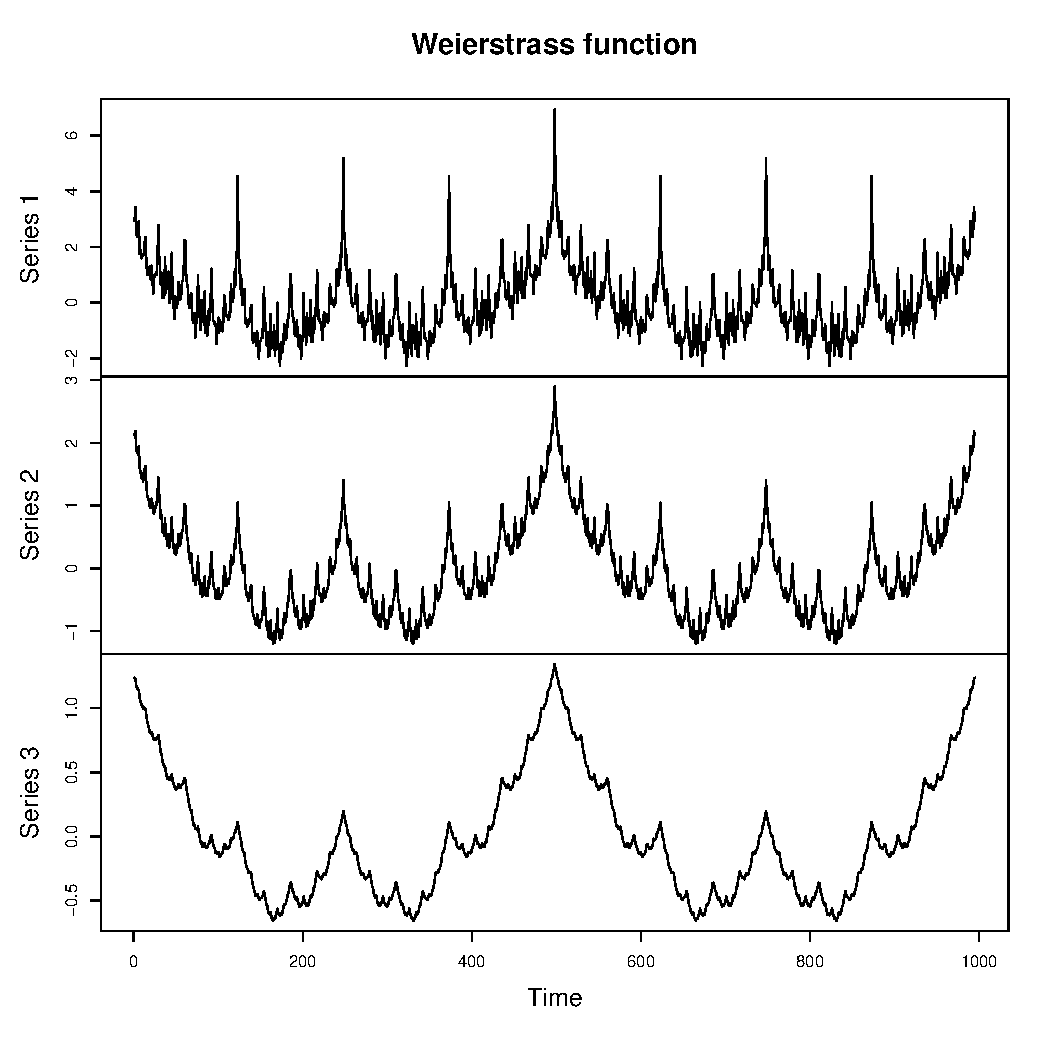
\includegraphics[width = 0.9\linewidth, height = 3in]{./figs/holder_notrandom-weier-notrandom.pdf}
    % \caption{Functions without added noise.}
    \label{fig:weierstrass}
  \end{subfigure}
  \hfill
  \begin{subfigure}[b]{0.49\textwidth}
  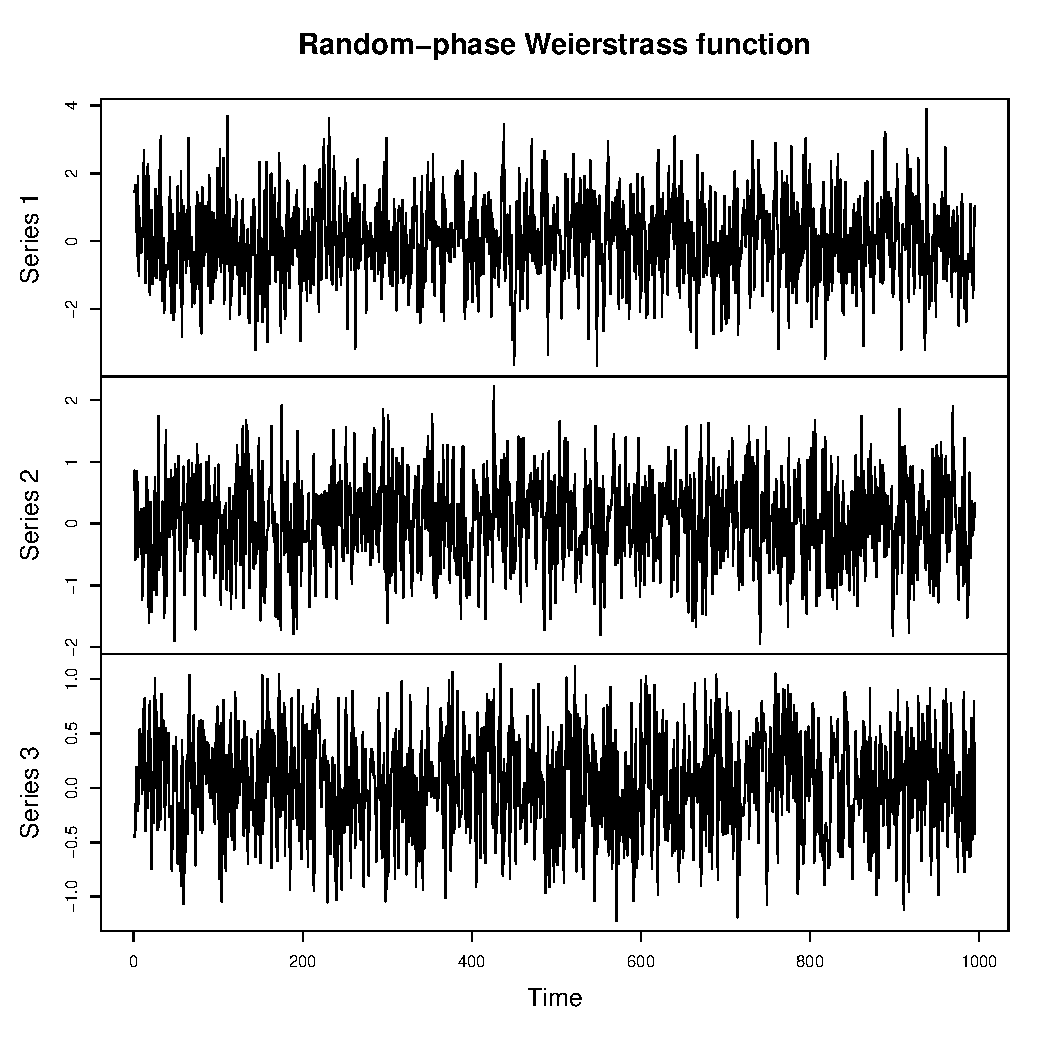
\includegraphics[width = 0.9\linewidth, height = 3in]{./figs/holder_coeffs-weier-random.pdf}
    % \caption{Functions without added noise.}
  \end{subfigure}
  \caption{The Weierstrass and random-phase Weierstrass function
  for $\alpha = \{ 0.20, 0.42, 0.80 \}$}
    \label{fig:weierstrass}
\end{figure}

\begin{figure}[!htbp]
  \begin{center}
  % \begin{picture}(60,60)
  % ./figs/coeff-interp-simple-functions1.pdf
  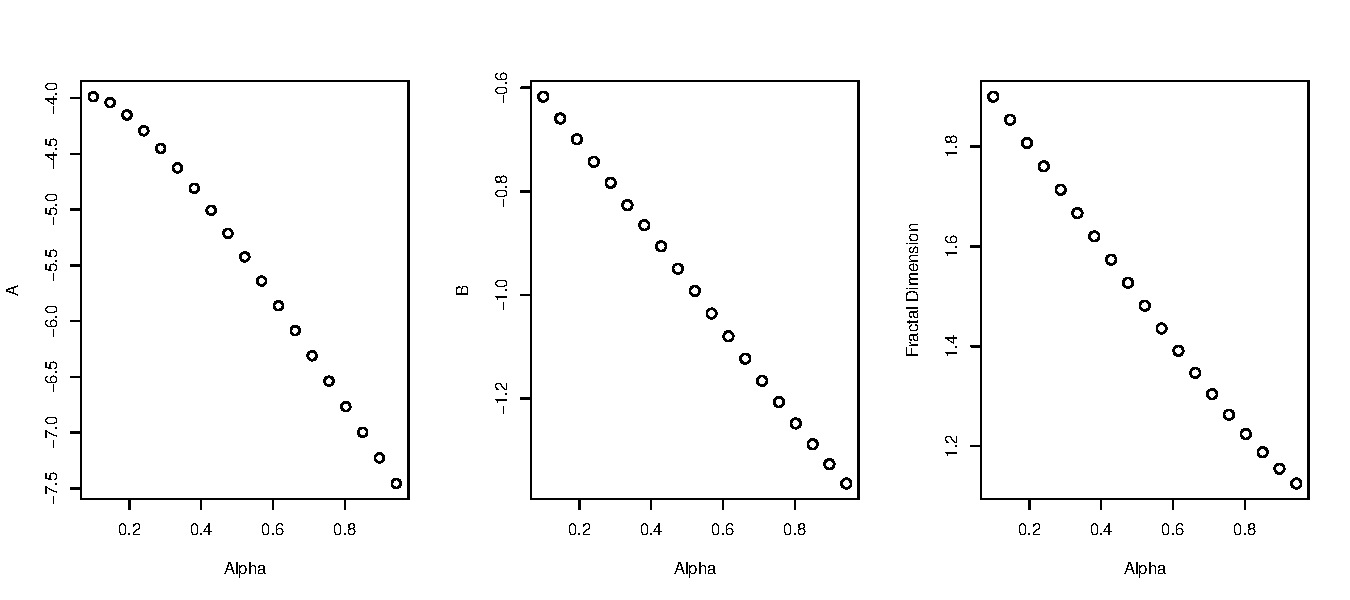
\includegraphics[width = \textwidth, keepaspectratio]{./figs/holder_notrandom-param-plots-notrandom}
  % \end{picture}
  \end{center} 
  \caption{Complexity coefficients and fractal dimension 
  plotted against the Weierstrass functions $\alpha$ parameter.  }
  \label{fig:notrandom-params}
\end{figure}


% \begin{figure}[!htbp]
%   \begin{center}
%   % \begin{picture}(60,60)
%   \includegraphics[height = 10cm,width = 10cm, keepaspectratio]
%   {./figs/holder_notrandom-fd-vs-B.pdf}
%   % \end{picture}
%   \end{center}
%   \caption{The complexity coefficients $B$ of the Weierstrass 
%   function 
%   plotted against the variogram estimate of fractal dimension.}
%   \label{fig:notrandom-B-fd} 
% \end{figure}

The  Weierstrass function written
\[
  W_{\alpha}(x) 
  \hspace{1em}= \sum_{n = 0}^{\infty} b^{-n \alpha} \cos(b^n \pi x).
\]
is H\"older $\alpha$ for $0 < \alpha < 1$ and has box-counting dimension $D-\alpha$.  
% The parameter $\alpha$ of the Weierstrass function 
% anhe 
% H\"older class and fractal dimension of the functions --  
% box-counting dimension for the deterministic 
For the random-phase Weierstrass function, as proved by Hunt\cite{hunt1998}, 
the parameter $\alpha$ determines the Hausdorff dimension of its graph. 
The two functions are illustrated in Figure \ref{fig:weierstrass} 
for three different paramaeter values $
\alpha = \{ 0.20, 0.42, 0.80 \}$. 
For smaller $\alpha$ the fractal dimension $D$ of the 
graphs increase.

Figure \ref{fig:notrandom-params} shows the change
in the complexity coefficients $A$ and $B$ and the
variogram fractal estimator $\hat D$ as the parameter 
$\alpha$ is varied. The relation of both the 
complexity coefficient $B$ and fractal estimator $\hat D$ to 
$\alpha$ is linear. For the complexity intercept 
$A$ there is some non-linear change for low values of $\alpha$. The fractal estimator 
$\hat D$ closely tracks the theoretical fractal. 

% Figure \ref{fig:notrandom-B-fd}
% shows that the complexity coefficient $B$ changes 
% linearly with the fractal estimator $\hat D$. 

The results for the Weierstrass function are deterministic, 
so the results shown are for a single estimate for 
each parameter.
The remaining functions are stochastic so the same 
the test was run on fifty samples functions or simulations the
estimated complexity coefficients and fractal dimension 
estimate are displayed as box plots to shown the distribution
of the estimates.

% ===============a=========================================
%  Holder, fBM and Cauchy section
% ========================================================
% holder_coeffs-weier-random.pdf
% alpha = 0.1936842 0.4278947 0.8026316
For the random-phase Weierstrass function Figure 
\ref{fig:rp-weierstrass-boxplot} shows there 
was no relationship between the change in the $\alpha$ 
parameter and the complexity coefficient $B$ or 
fractal estimator $\hat D$. The intercept coefficient $A$ increases 
linearly but the total magnitude of the change is 
relatively small-- the median of the estimates has a range 
of less than $0.5$. The 
reported results were for simulations of 2000 
points. The simulation was repeated at for lengths between 
500 and 2000 but the returned the same results. We 
do not have an explanation for the discrepancy between 
the theoretical H\"older class and fractal dimension 
of the function and the results of the simulation. Unlike the determinstic Weierstrass 
function and the Cauchy and Fractional Brownian 
motion processes, the graph of the random-phase 
Weierstrass did not become locally smoother as 
$\alpha$ was increased and the coefficient $B$ and 
estimator $\hat D$ are numerically similar to the results 
given when white noise was added to the simple functions 
as reported in Table \ref{tab:simple-coeffs}.

\begin{figure}[!htbp]
  \begin{center}
  % \begin{picture}(60,60)
  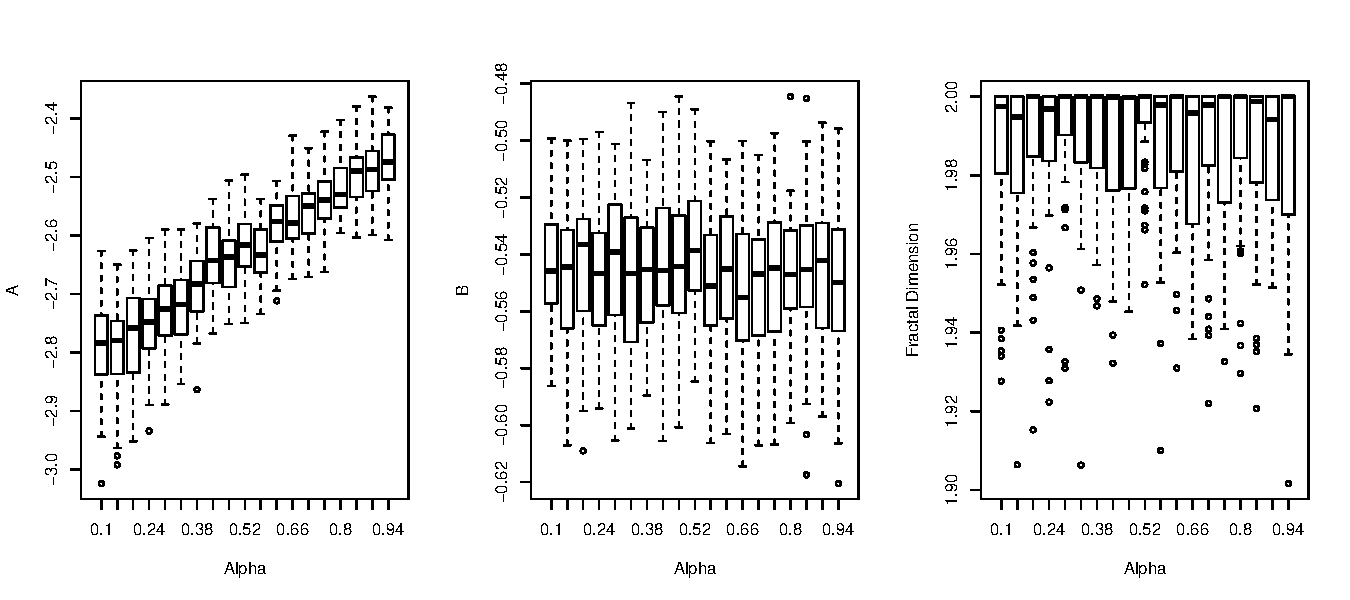
\includegraphics[height = 3in, width =6in, keepaspectratio]{./figs/holder_coeffs-boxplots.pdf}
   
  \caption{Complexity coefficients and fractal dimension 
  plotted against the $\alpha$ parameters of the 
  random-phase Weierstrass function.  }
  % \end{picture}
    \label{fig:rp-weierstrass-boxplot}
  \end{center}
\end{figure}

Examples of the FBM and Cauchy process time series used in our simulation are shown in figure \ref{fig:cauchyplot}. 
The results are similar to those of the deterministic 
Weierstrass function and both the complexity coefficient 
$B$ and $\hat D$ change linearly with the H\"older class
parameter. Also similar to the results for the Weierstrass 
function, the coefficient $A$ has a non-linear relation to $\alpha$.  
\begin{figure}[!htbp]
  \begin{subfigure}[b]{0.49\textwidth}
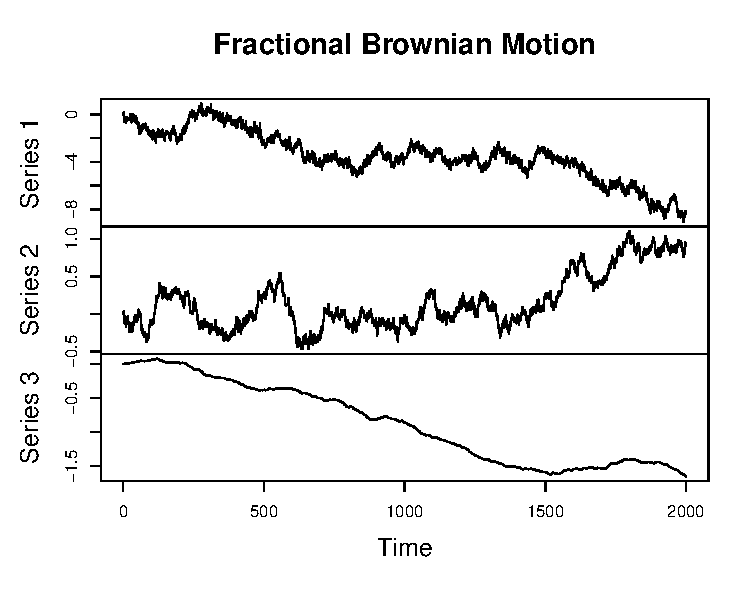
\includegraphics[width = 0.9\linewidth, height = 3in]{./figs/fBm-coeffs-plot.pdf}
    % \caption{Functions without added noise.}
    % \label{fig:fBmplot}
  \end{subfigure}
  \hfill
  \begin{subfigure}[b]{0.49\textwidth}
  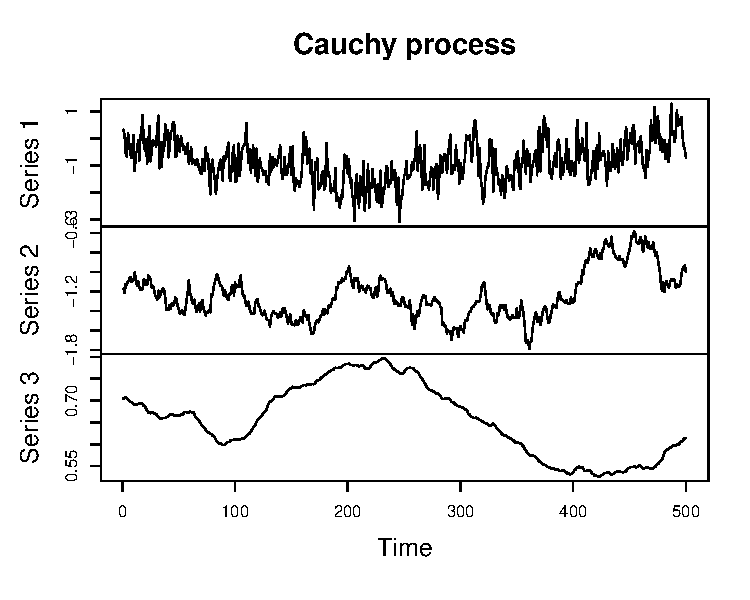
\includegraphics[width = 0.9\linewidth, height = 3in]{./figs/cauchy-plot.pdf}
    % \caption{Functions without added noise.}
    
  \end{subfigure}
  
  \caption{Fractional Brownian motion and the Cauchy process with $\alpha = \{ 0.20, 0.42, 0.80 \}$. The Cauchcy $\beta$ parameter was 
  held constant.}
  \label{fig:cauchyplot}
\end{figure}

\begin{figure}[!htbp]
  \begin{center}
  % \begin{picture}(60,60)
  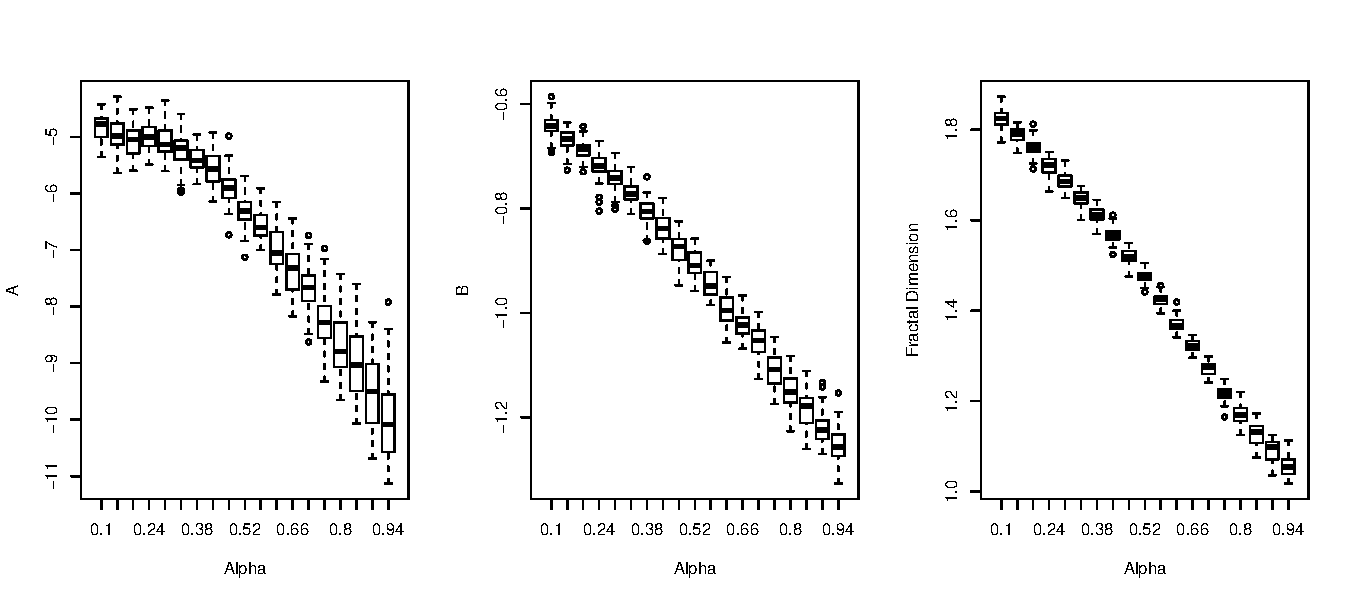
\includegraphics[height = 3in, width =6in, keepaspectratio]{./figs/fBm-coeffs-boxplots.pdf}
  % \end{picture}
  \end{center}
   \label{fig:fbm-boxplots}
  \caption{Complexity coefficients and fractal dimension plotted against the $\alpha$ coefficients of fractional Brownian motion.} 
\end{figure}

\begin{figure}[!htbp]
  \begin{center}
  % \begin{picture}(60,60)
  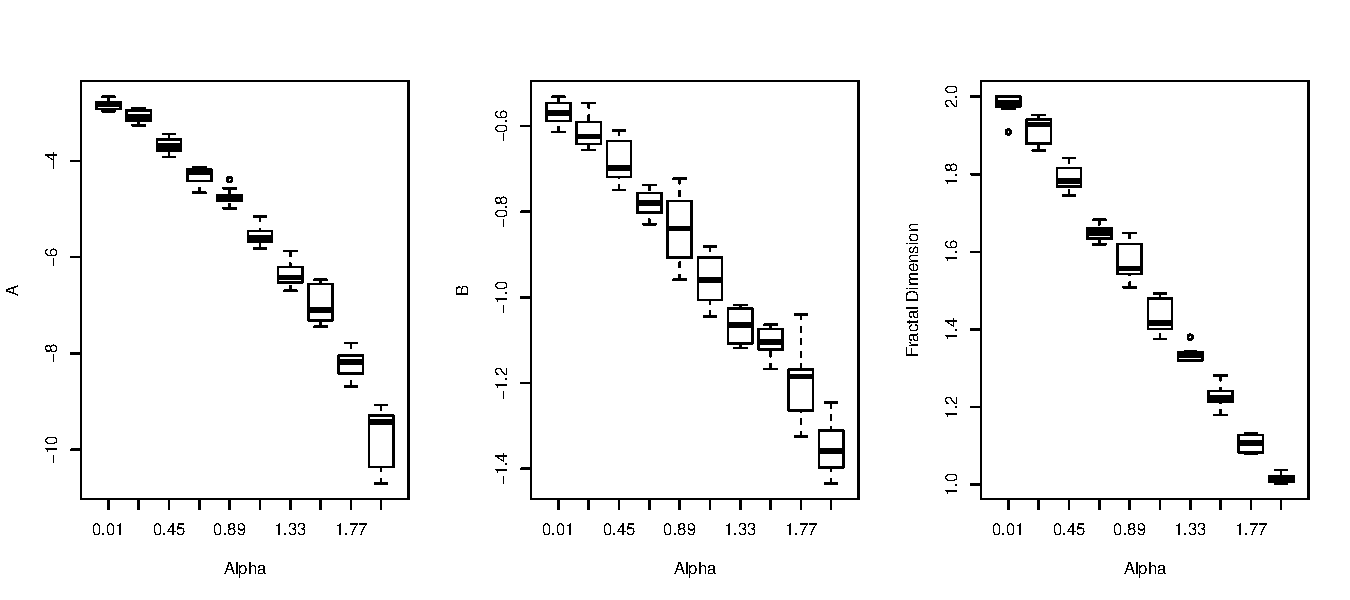
\includegraphics[height = 3in, width =6in, keepaspectratio]{./figs/cauchy-boxplots.pdf}
  % \end{picture}
  \end{center}
  \caption{Complexity coefficients and fractal dimension plotted against the Cauchy process $\alpha$ coefficient.} 
     \label{fig:cauchy-boxplots}
\end{figure}

The Cauchy process has two parameters, $\alpha$ determines
fractal dimension and the parameter $\beta$ determines 
the Hurst coefficient, or the long range correlation of the 
process. 20 simulations of the Cauchy process were generated
on a $10 \times 10$ grid of parameters $\alpha, \beta$
for $0 < \alpha < 2$ and $0 < \beta < 1.5$. 
In figure \ref{fig:cauchy-alpha} plots the mean value of the complexity coefficients as the long-range parameter 
$\alpha$ changes. Differences in the $\beta$ parameter show no effect the estimate of the complexity coefficients or the fractal estimator. 

\begin{figure}[!htbp]
  \begin{center}
  % \begin{picture}(60,60)
  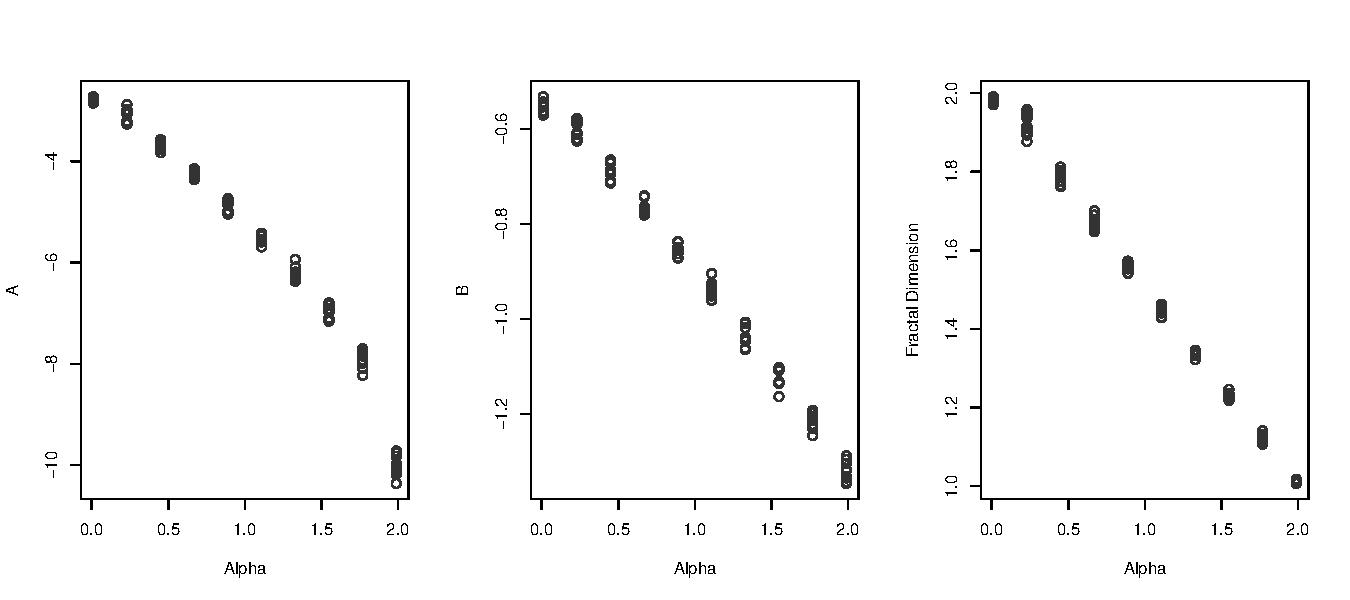
\includegraphics[height = 3in, width =6in, keepaspectratio]{./figs/cauchyalpha-scatterplots.pdf}
  % \end{picture}
  \end{center}
  \caption{The mean value of the complexity coefficients and fractal dimension plotted against the Cauchy process $\alpha$ coefficient.}
   \label{fig:cauchy-alpha}
\end{figure}

\begin{figure}[h]
  \begin{center}
  % \begin{picture}(60,60)
  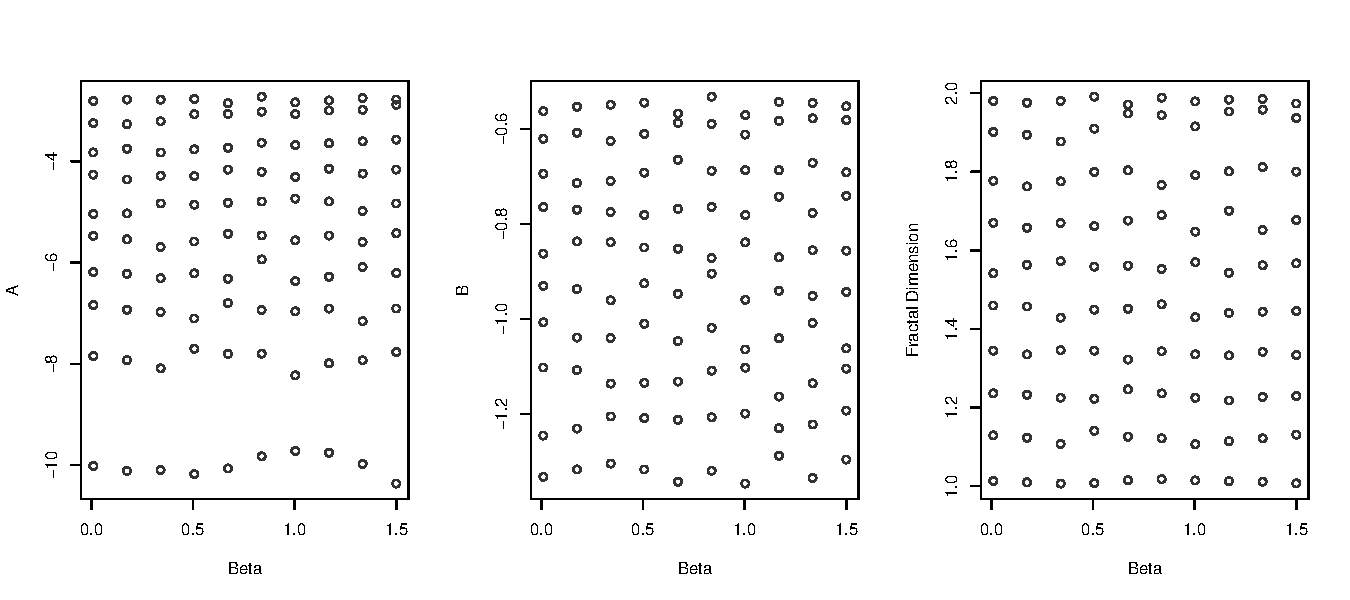
\includegraphics[height = 3in, width =6in, keepaspectratio]{./figs/cauchybeta-scatterplots.pdf}
  % \end{picture}
  \end{center}
  \caption{The mean value of the omplexity coefficients and fractal dimension plotted against the Cauchy process $\beta$ coefficient.}
 \label{fig:cauchy-beta}
\end{figure}

Figure \ref{fig:cauchy-beta} shows another view of 
the complexity coefficients plotted against 
changes the Cauchy process parameter $beta$. The complexity 
coefficient $B$ and fractal dimension clearly preserve 
the grid from the parameter space -- for a fixed 
$\beta$, the parameter varies linearly with $\alpha$. The 
$\beta$ parameter controls the long-range dependence of 
the Cauchy process and the plots indicate that 
the complexity coefficients, like fractal dimension,
measure a local, not global, property of a function.


Although these results are intended to be exploratory, for 
three of the four functions there is strong evidence that
the complexity coefficient $B$ behaves similarly to the 
variogram estimator of fractal dimension. The complexity 
coefficient $A$ does not seem to add much information 
for the three cases in which there was a linear relation between 
 $B$, $\hat D$, and the parameter determining the 
 H\"older exponent of the function, $\alpha$. 
 On the other hand, our initial example of simple functions and the random-phase Weierstrass functions appears shows a relationship between the intercept 
coefficient $A$ and fine-scale noise. These results are for a small set of processes with well-known behavior. A comparison of the complexity coefficient $B$ and fractal estimators on a wider variety of time series might show whether this relation holds under a wider range of conditions.





















